\documentclass[lettersize,journal]{IEEEtran}
\usepackage{amsmath,amsfonts}
\usepackage{algorithmic}
\usepackage{algorithm}
\usepackage{array}
\usepackage[caption=false,font=normalsize,labelfont=sf,textfont=sf]{subfig}
\usepackage{textcomp}
\usepackage{stfloats}
\usepackage{url}
\usepackage{verbatim}
\usepackage{graphicx}
\usepackage{cite}
\usepackage{color}
\hyphenation{op-tical net-works semi-conduc-tor IEEE-Xplore}
% updated with editorial comments 8/9/2021

\definecolor{mygray}{gray}{0.6}
\definecolor{myblue}{rgb}{0.8,0.85,1} 


\newcommand{\defequal}{\mbox{$\stackrel{\triangle}{=}$}}
\DeclareMathOperator{\vecOp}{\mathrm{vec}}
\DeclareMathOperator{\tr}{\mathrm{tr}}
\DeclareMathOperator{\E}{\mathbb{E}}
\DeclareMathOperator{\var}{\mathbb{V}\mathrm{ar}}
\DeclareMathOperator{\cov}{\mathrm{Cov}}
\DeclareMathOperator{\sgn}{\mathrm{sgn}}
\DeclareMathOperator{\etr}{\mathrm{etr}}
\DeclareMathOperator{\re}{\mathfrak{Re}}
\DeclareMathOperator{\im}{\mathfrak{Im}}

\newcommand{\B}[1]{{\pmb{#1}}}
\newcommand{\FN}[1]{\left\|{#1}\right\|_\mathrm{F}}
\newcommand{\MGF}[2]{\phi_{#1}\left({#2}\right)}
\newcommand{\EXs}[2]{\E_{{#1}}\left\{{#2}\right\}}
%\newcommand{\PDF}[2]{f_{{#1}}\left({#2}\right)}
%\newcommand{\CDF}[2]{F_{{#1}}\left({#2}\right)}
\newcommand{\ERV}[1]{\Upsilon\left({#1}\right)}
\newcommand{\Bessel}[2]{\mathcal{K}_{{#1}}\left({#2}\right)}
\newcommand{\ExpInt}[2]{\mathrm{Ei}_{{#1}}\left({#2}\right)}

\newcommand{\conv}{\mbox{conv}}
\newcommand{\ds}{\displaystyle}
%Huy commands definition
\newcommand{\clS}{{\cal S}}
\newcommand{\clA}{{\cal A}}
\newcommand{\clB}{{\cal B}}
\newcommand{\clC}{{\cal C}}
\newcommand{\clD}{{\cal D}}
\newcommand{\clP}{{\cal P}}
\newcommand{\clR}{{\cal R}}
\newcommand{\clM}{{\cal M}}
\newcommand{\clN}{{\cal N}}
\newcommand{\clL}{{\cal L}}
\newcommand{\clH}{{\cal H}}
\newcommand{\clK}{{\cal K}}
\newcommand{\clE}{{\cal E}}
\newcommand{\clF}{{\cal F}}
\newcommand{\clI}{{\cal I}}
\newcommand{\clT}{{\cal T}}
\newcommand{\clO}{{\cal O}}
\newcommand{\clU}{{\cal U}}
\newcommand{\clW}{{\cal W}}
\newcommand{\wei}{{\boldsymbol{\theta}}}
\newcommand{\weitar}{{\wei"}}
\newcommand{\dfactor}{\gamma}
\newcommand{\lrate}{\beta}
\newcommand{\emax}{e^{max}}
\newcommand{\bz}{\mathbf{z}}
\newcommand{\ba}{\mathbf{a}}
\newcommand{\bc}{\mathbf{c}}
\newcommand{\be}{\mathbf{e}}
\newcommand{\bs}{\mathbf{s}}
\newcommand{\bh}{\mathbf{h}}
\newcommand{\bg}{\mathbf{g}}
\newcommand{\bA}{\mathbf{A}}
\newcommand{\bB}{\mathbf{B}}
\newcommand{\bC}{\mathbf{C}}
\newcommand{\bV}{\mathbf{F}}
\newcommand{\bVi}{\widetilde{\mathbf{V}}}
\newcommand{\bW}{\mathbf{W}}
\newcommand{\bI}{\mathbf{I}}
\newcommand{\bJ}{\mathbf{J}}
\newcommand{\bH}{\mathbf{H}}
\newcommand{\bG}{\mathbf{G}}
\newcommand{\bX}{\mathbf{X}}
\newcommand{\bY}{\mathbf{Y}}
\newcommand{\bN}{\mathbf{N}}

\newcommand{\bx}{\mathbf{x}}
\newcommand{\bw}{\mathbf{w}}
\newcommand{\bxc}{\mathbf{x}^c}
\newcommand{\bxr}{\mathbf{x}^r}
\newcommand{\by}{\mathbf{y}}
\newcommand{\bt}{\mathbf{t}}
\newcommand{\bn}{\mathbf{n}}
\newcommand{\bp}{\mathbf{p}}
\newcommand{\bnc}{\mathbf{n}^c}
\newcommand{\bnr}{\mathbf{n}^r}
\newcommand{\bv}{\mathbf{f}}

\newcommand{\bvr}{\mathbf{v}^r}
\newcommand{\bvc}{\mathbf{v}^c}
\newcommand{\bVr}{\mathbf{V}^r}
\newcommand{\bVc}{\mathbf{V}^c}
\newcommand{\bff}{\mathbf{f}}
\newcommand{\blam}{\boldsymbol{\lambda}}
\newcommand{\bgam}{\boldsymbol{\gamma}}
\newcommand{\tpri}{T_{PRP}}
\newcommand*{\h}{^{\mathsf{H}}}
\newcommand{\noise}{\sigma^2}
\newcommand{\iu}{\rm{IU}}
\newcommand{\pu}{\rm{PU}}
\newcommand{\su}{\rm{SU}}
\newcommand{\eu}{\rm{EU}}
\newcommand{\dd}{\rm{D2D}}
\newcommand{\D}{\mathcal{D}}
\newcommand{\tc}{\bar{\mathbf{t}}}
\newcommand{\ti}{t_{\rm{I}}}
\newcommand{\te}{t_{\rm{E}}}
\newcommand{\td}{t_d}
\newcommand{\T}{^{\rm{T}}}
\newcommand{\tni}{\bar{t}_{\rm{I}}}
\newcommand{\tne}{\bar{t}_{\rm{E}}}
\newcommand{\tnd}{\tau_d}
\newcommand{\tnik}{\bar{t}_{\rm{I}}^{\langle l \rangle}}
\newcommand{\tnek}{\bar{t}_{\rm{E}}^{\langle l \rangle}}
\newcommand{\tndk}{\tau_d^{\langle l \rangle}}
\newcommand{\pgs}{p}
\newcommand{\igs}{i}
\newcommand{\sinr}{\gamma}
\newcommand{\amp}{\alpha}
\newcommand{\ang}{\theta}
\newcommand{\la}{\langle}
\newcommand{\ra}{\rangle}

\newcommand{\Vik}{\widetilde{\mathbf{F}}^{\langle l \rangle}}
\newcommand{\vk}{\mathbf{f}^{\langle l \rangle}}
\newcommand{\ck}{\mathbf{c}^{\langle l \rangle}}
\newcommand{\ckk}{\mathbf{c}^{\langle l+1 \rangle}}
\newcommand{\wk}{\mathbf{w}^{\langle l \rangle}}
\newcommand{\Vk}{\mathbf{F}^{\langle l \rangle}}
\newcommand{\Wk}{\mathbf{W}^{\langle l \rangle}}
\newcommand{\pk}{p^{\langle l \rangle}}
\newcommand{\tauk}{\bar{\mathbf{t}}^{\langle l \rangle}}
\newcommand{\vkk}{\mathbf{f}^{\langle l+1 \rangle}}
\newcommand{\wkk}{\mathbf{w}^{\langle l+1 \rangle}}
\newcommand{\Vkk}{\mathbf{F}^{\langle l+1 \rangle}}
\newcommand{\Wkk}{\mathbf{W}^{\langle l+1 \rangle}}

\newcommand{\pkk}{p^{\langle l+1 \rangle}}
\newcommand{\zk}{z^{\langle l \rangle}}
\newcommand{\taukk}{\bar{\mathbf{t}}^{\langle l+1 \rangle}}
\newcommand{\brc}{\boldsymbol{\Theta}}
\newcommand{\brcv}{\boldsymbol{\theta}}
\newcommand{\rcvk}{\boldsymbol{\theta}^{\langle l \rangle}}
\newcommand{\rcvkk}{\boldsymbol{\theta}^{\langle l+1 \rangle}}
\newcommand{\bamp}{\boldsymbol{\alpha}}
\newcommand{\btau}{\bar{\mathbf{t}}}
\newcommand{\brho}{\boldsymbol{\rho}}
\newcommand{\hok}{\boldsymbol{\rho}^{\langle l \rangle}}
\newcommand{\hokk}{\boldsymbol{\rho}^{\langle l+1 \rangle}}



\begin{document}



\title{A Secure PolyDot Matrix Multiplication Approach For Distributed Computing}

\author{
        % <-this % stops a space
\thanks{}% <-this % stops a space
\thanks{}}

% The paper headers
%\markboth{Journal of \LaTeX\ Class Files,~Vol.~14, No.~8, August~2021}%
%{Shell \MakeLowercase{\textit{et al.}}: A Sample Article Using IEEEtran.cls for IEEE Journals}

%\IEEEpubid{0000--0000/00\$00.00~\copyright~2021 IEEE}
% Remember, if you use this you must call \IEEEpubidadjcol in the second
% column for its text to clear the IEEEpubid mark.

\maketitle

\begin{abstract}

\end{abstract}

\begin{IEEEkeywords}

\end{IEEEkeywords}



%%%%%%%%%%%%%%%%%%%%%%%%%%%%%%%%%%%%%%%%%%
\section{System Models}
\begin{figure*}[!h]
 \centering
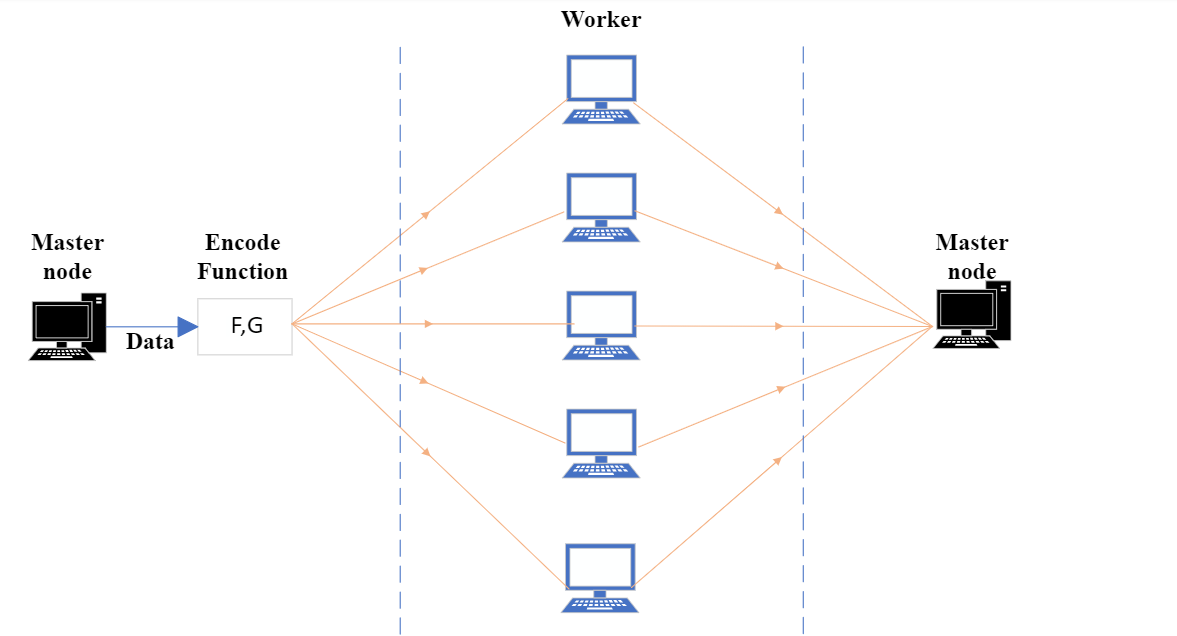
\includegraphics[width=0.7\linewidth]{fig/Distributed computing system.png}
    \captionsetup{justification=centering} 
 \caption{General overview of distributed computing systems.
}
  \label{Encode example}
\end{figure*}
\subsection{Symbolism}
Before delving into the discussion of the system model, we would like to present some commonly used symbols that will be employed consistently throughout.We use uppercase letters (A, B, X, Y, ...) to denote matrices. A sufficiently large finite Galois field of size $|\mathbb{F}|$ is denoted as $\mathbb{F}$. With a real number a, let $\left\lceil a\right\rceil$ denote the ceiling function of a, which is the smallest integer greater than or equal to a. I(X) can be considered as a function used to quantify the amount of information gained with respect to the event X.
\begin{equation}
    I(X) = -log_2(P(X))
\end{equation}.
 We also represent $I(X, Y)$ as the amount of mutual information between two variables X and Y.\\
The function $H(X)$ is the information entropy function for the parameter X, understood as the measure of uncertainty that information carries that can be represented as:
\begin{equation}
    H(X) = - \sum_{i} P(x_i) \log_2(P(x_i))
\end{equation}
with $P(x_i)$ is the probability of the event $x_i \in X$. Additionally, we have the following definitions: $H(X,Y)$ represents information contained in the pair $(X, Y)$, and $H(X|Y$
 represents the information in X that is not present in Y. From here, we have related expressions for I and H as follows:
\begin{equation}
    I(X,Y) = I(Y,X) = H(X) - H(X|Y)
                    = H(Y) - H(Y|X)
 \end{equation}

For distributed computing systems, we denote the number of workers as N,
 $R_c$ as the minimum recovery threshold or the minimum number of workers necessary to recover the result, $P_C$ as the number of colluding workers, B as the set of Byzantine workers (The definitions of colluding worker and Byzantine worker will be introduced in the following section) and $C_l$ as the communication load defined as as the quantity of information retrieved from the workers.






\subsection{PolyDot Code without security}

\begin{itemize}
\item m = t , n = s , p = d
\end{itemzie}


In this section, we will introduce a coded distributed matrix-matrix multiplication problem, named PolyDot. This method represents a trade-off between recovery threshold and communication load compared to Polynomial Code and MatDot Code. Master node needs compute Z = AB, where X,Y are data matrices, we also assume that the number of colluding workers and the number of Byzantine workers are 0. First, master node partition the matrix  \( X \in \mathbb{F}^{M \times N } \)  and \(Y \in\mathbb{F}^{N \times P}\)
 into submatrices as shown below:
\[
\begin{array}{cc}
X = \left[ \begin{array}{cccc}
X_{1,1}  & \ldots & X_{1,n} \\

\vdots  & \ddots & \vdots \\
X_{m,1}  & \ldots & X_{m,n} \\
\end{array} \right]
&
Y = \left[ \begin{array}{cccc}
Y_{1,1}  & \ldots & Y_{1,p} \\
\vdots &\ddots & \vdots \\
Y_{n,1}  & \ldots & Y_{n,p} \\
\end{array} \right]
\end{array}
\]
where \(m \mid M, n \mid N, p \mid P \), \(X_{i,j} \in \mathbb{F}^{\frac{M}{m} \times \frac{N}{n}} \), 
\(Y_{k,l} \in \mathbb{F}^{\frac{N}{n} \times \frac{P}{p}} \)
The resulting matrix Z = XY is represented as follows:
\[
Z = \begin{bmatrix}
Z_{1,1}  & \ldots & Z_{1,p} \\

\vdots & \ddots & \vdots \\
Z_{m,1}  & \ldots & Z_{m,p} \\
\end{bmatrix}
\]
with \(Z_{u,v}\) = \(\sum_{k=1}^{n} X_{u,k}Y_{k,v}\), \( u \in \{1,2,\ldots, m\} \), \( v \in \{1,2,\ldots, p\} \) 


\subsubsection{Encode}
The Master node encodes the submatrices of X and Y using the functions \(F\) and \(G\) below:  
\begin{equation}
F(z)  = \sum_{i=1}^{m} \sum_{j=1}^{n} X_{i,j}z^{n(i-1)+j-1}
\end{equation}
\begin{equation}
G(z)  = \sum_{k=1}^{n} \sum_{l=1}^{p} Y_{k,l}z^{n-k+mn(l-1)}
\end{equation}

where \(F \) and \(G \)are encode function satisfied \(F : \mathbb{F}^{\frac{M}{m} \times \frac{N}{n}} \rightarrow \mathbb{F}^{\frac{M}{m} \times \frac{N}{n}} \) and \(G : \mathbb{F}^{\frac{N}{n} \times \frac{P}{p}} \rightarrow \mathbb{F}^{\frac{N}{n} \times \frac{P}{p}} \).
Subsequently, the master node sends to the i-th worker the expressions \(F(z_i)\) and \(G(z_i)\) , where it is noted that \(z_i\) is distinct and non-zero for i \(  \in \) {1,2,...,p}

\subsubsection{Task computing} 
i-th worker calculate \(F(z_i)G(z_i) \).
As soon as worker \(i\) completes the computation, it will send the result back to the master node, noting that the returned results from the workers may vary in speed depending on each worker's computational capabilities, and the returned results may not be accurate.
\begin{equation}
\begin{aligned}
F(z)G(z) &= \left( \sum_{i=1}^{m} \sum_{j=1}^{n} X_{i,j}z^{n(i-1)+j-1} \right)  \\
&\quad \times \left( \sum_{k=1}^{n} \sum_{l=1}^{p} Y_{k,l}z^{n-k+mn(l-1)} \right) \\
&= \sum_{i,j,k,l}^{} X_{i,j}Y_{k,l}z^{n(i-1)+j-1+n-k+mn(l-1)}     \\
\end{aligned}


The coefficient of \(Z_{u,v}\) in the polynomial corresponding to the exponent z is \(n(u-1)+n-1+mn(v-1)\) in the case where the index j = k in \(X_{i,j}\) and \(Y_{k,l}\)

\subsubsection{Result recovering (Decoding)}
The master node will collect the fastest R results returned by the workers. Afterward, the master node will recover the result \(Z_{i,j}\)  with \( i \in \{1,2,\ldots, m\} \), \( j \in \{1,2,\ldots, p\} \)   based on polynomial interpolation.\\
   Since the degree of the polynomial is mnp + n - 2, when applying the polynomial interpolation method, a minimum of mnp + n - 1 values is required to achieve the fastest results from the workers for the recovery of the matrix 
Z. Therefore, the recovery threshold is:
\begin{equation}
\label{no label}
    P_R = mnp + n - 1
\end{equation}
and communication load is: 
\begin{equation}
   \label{communication_load}
    C_L = P_R\frac{MP}{mp}
\end{equation}

Example 1: m = 1, n = 2, p = 3
\[
\begin{array}{cc}
X = \left[ \begin{array}{cccc}
X_{1,1}  & X_{1,2} \\

\end{array} \right]
&
Y = \left[ \begin{array}{cccc}
Y_{1,1}  & Y_{1,2} & Y_{1,3} \\
Y_{2,1}  & Y_{2,2} & Y_{2,3} \\
\end{array} \right]
\end{array}
\]
\begin{equation}
Z = XY = \begin{bmatrix}
Z_{1,1}  & Z_{1,2} & Z_{1,3} \\

\end{bmatrix} 
\end{equation}
We define the encode funtion: 
\begin{align*}
F(z) &= \sum_{i=1}^{1} \sum_{j=1}^{2} X_{i,j}z^{2(i-1)+j-1} \\
&= X_{1,1} + X_{1,2}z \\
G(z)  &= \sum_{k=1}^{2} \sum_{l=1}^{3} Y_{k,l}z^{2-k+2*(l-1)} \\ 
&=Y_{1,1}z+Y_{1,2}z^{3}+Y_{1,3}z^{5}+Y_{2,1}+Y_{2,2}z^{2}+Y_{2,3}z^{6}
\end{align*}

Consider expression \(F_z\) = \(F(z)G(z)\): \\
\begin{comment}
The coefficient of z is: \(Z_{1,1}\) \\
The coefficient of \(z^{5}\) is: \(Z_{1,2}\)\\ 
The coefficient of \(z^{9}\) is: \(Z_{1,3}\) \\ 
The coefficient of \(z^{3}\) is: \(Z_{1,3}\)  \\
The coefficient of \(z^{7}\) is: \(Z_{2,2}\)  \\
The coefficient of \(z^{11}\) is: \(Z_{2,3}\) \\
\end{comment}
\\
\\

\begin{center}
\begin{tabular}{|>{\centering\arraybackslash}m{4em}|>{\centering\arraybackslash}m{4em}|}
   \hline
   Coefficient  &  Exponent of $z$  \\ \hline
   $Z_{1,1}$  &      1 \\
   $Z_{1,2}$  &      3 \\
   $Z_{1,3}$  &      5 \\\hline
\end{tabular} 
\end{center}
\\\

Retrieve distinct points \(z_1, z_2, ... z_p \) with \( z_i \in \mathbb{F}, \) $i \in \{1, \ldots, P\}$. Then, master node send \(F(z_i)\)and \(G(z_i)\) to ith-worker i. Then, i-th worker  will compute \(F(z_i)G(z_i)\) and send the result back to the master node. Because the highest degree of the polynomial\(F_z\) is 11, it is necessary to have a minimum of 12 equations to determine the polynomial \(F_z\), or in other words, to calculate its coefficients. When the fastest 12 nodes complete the computation and return the results, the master node will restore the coefficients \(Z_{u,v}\) of matrices Z using polynomial interpolation.\\

\textbf{Remark:} 
The PolyDot code method presented above represents a trade-off between recovery threshold and communication load. However, in practical distributed computing systems, issues related to malicious workers and colluding workers are common challenges. Malicious (Byzantine) workers may provide deliberately incorrect computations to sabotage the overall computation results, while colluding workers, typically located at edge nodes, collaborate to share information gathered from the input data. The Polydot Code mentioned above is not designed to withstand colluding workers as well as Byzantine workers. Therefore, in the following section, we will introduce the Secure PolyDot Code (SPC), which addresses both colluding worker and Byzantine worker scenarios.


\section{PolyDot with Security.}
\begin{figure*}[!h]
 \centering
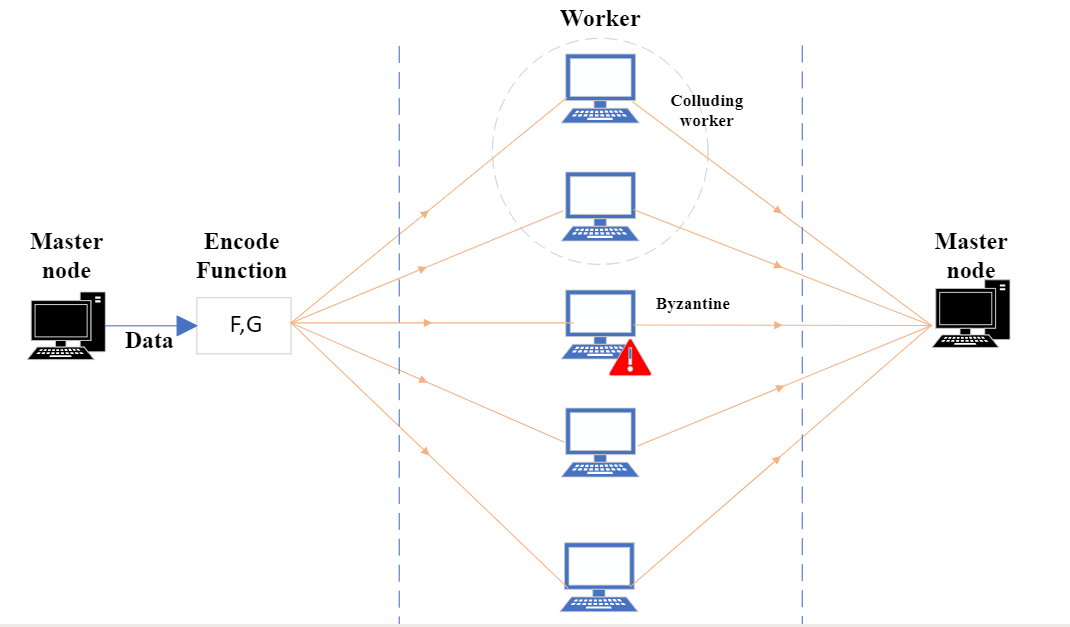
\includegraphics[width=0.7\linewidth]{fig/Colluding and Byzantine wc.png}
 \caption{A description of a distributed computing system with security issues. Due to varying computational capabilities and different return times for results from individual workers, the overall computation time of the master node is affected. Colluding workers may share information to obtain data details, while some workers might intentionally send inaccurate results with the goal of distorting the final outcome.}
  \label{Security in edge computing}
\end{figure*}
\subsection{Generalized Polydot with Security}
In the preceding section, we analyzed the PolyDot code under the assumption of an absence of colluding and malicious workers. Nevertheless, in practical scenarios, colluding workers may conspire to exchange information, and malicious workers might provide inaccurate results, thereby influencing the computational process of the master node with deviations. Consequently, in this section, we present the Secure PolyDot Code (SPC) as a solution to mitigate the impact of colluding workers and malicious workers. SPC is carried out as follows:
\subsubsection{Encode} To accomplish this objective, we add rows or columns containing random elements to matrices A and B, respectively. From there, we consider two distinct cases:

\textbf{a) Case: $n < m$:}

 First, we defination:
\[
\Delta_{P_C} = \left\lceil\frac{P_C}{n}\right\rceil
\]
Matrix \(X^* \) will be represented:
\[
X^* =
\begin{bmatrix}
X_{1,1} & \ldots & X_{1,n} \\
\vdots & \ddots & \vdots \\
X_{m,1} & \ldots & X_{m,n} \\
R_{1,1} & \ldots & R_{1,n} \\
\vdots & \ddots & \vdots \\
R_{\Delta_{P_C},1} & \ldots & R_{\Delta_{P_C},s}
\end{bmatrix}
\label{eq:matrixA}
\]
while the $n \times p^*$ augmented matrix $Y^* = [Y \ R_0]$ with $p^* = p + \Delta_{P_C}$ is obtained as
\[
Y^* =
\begin{bmatrix}
Y_{1,1} & \ldots & Y_{1,p} & R_{n,1} & \ldots & R_{n,\Delta_{P_C}} \\
\vdots & \ddots & \vdots & \vdots & \ddots & \vdots \\
Y_{n,1} & \ldots & Y_{n,p} & Y_{1,1} & \ldots & R_{1,\Delta_{P_C}}
\end{bmatrix}
\label{eq:matrixB}
\]
\\
The encoding functions \(F^*\) and \(G^*\) are rewritten as follows:
\begin{equation}
\begin{aligned}
\label{encode_1}
F^*(z) = \sum_{i=1}^{m} \sum_{j=1}^{n} X_{i,j}^* z^{n(i-1)+(j-1)} + \sum_{i=m+}^{m^*} \sum_{j=1}^{n} X_{i,j}^* z^{n(i-1)+j-1}
\end{aligned}
\end{equation}
\begin{equation}
\begin{aligned}
\label{encode_2}
G^*(z) &= \sum_{k=1}^{n} \sum_{l=1}^{p} Y_{k,l}^* z^{n-k+m^*n(l-1) } \\
&\quad + \sum_{k=1}^{n} \sum_{l=p+1}^{p^*} Y_{k,l}^* z^{m^*np+n(l-p)-k}
\end{aligned}
\end{equation}

% The s ≥ t Case
\textbf{b) Case: $n \geq m$:}

\[
\Delta_{P_C} =\left\lceil \frac{P_C}{\min\{m, p\}} \right\rceil
\]
 Matrix $X^* \in \mathbb{F}^{t\times n^*}   $  will take the form $[X \ R] $ with $n^* = n + \Delta_{P_C}$ is obtained as
\[
X^* =
\begin{bmatrix}
X_{1,1} & \ldots & X_{1,n} & R_{1,1} & \ldots & R_{1,\Delta_{P_C}} \\
\vdots & \ddots & \vdots & \vdots & \ddots & \vdots \\
X_{m,1} & \ldots & X_{m,n} & X_{m,1} & \ldots & R_{m,\Delta_{P_C}}
\end{bmatrix}
\]
and the matrix $Y^* = [R \ Y] \in \mathbb{F}^{n^*\times d} $ is represented as:
\[
Y^* =
\begin{bmatrix}
R_{\Delta_{P_C},1} & \ldots & R_{\Delta_{P_C},p} \\
\vdots & \ddots & \vdots \\
R_{1,1} & \ldots & R_{1,p} \\
Y_{1,1} & \ldots & Y_{1,p} \\
\vdots & \ddots & \vdots \\
Y_{n,1} & \ldots & Y_{n,p}
\end{bmatrix}
\]
And the encoding function in this case will be represented: 
\begin{equation}
    \begin{aligned}
    \label{encode_3}
        F^*(z) &= \sum_{i=1}^{m} \sum_{j=1}^{n} X_{i,j}^* z^{i-1 + m(j-1)} \\
        &\quad + \sum_{i=1}^{m} \sum_{j=n+1}^{n^*} X_{i,j}^* z^{i-1 + m(j-1)}, \\
         \end{aligned}
\end{equation}
\begin{equation}
    \begin{aligned}
    \label{encode_4}
        G^*(z) &= \sum_{k=1+\Delta_{P_C}}^{p} \sum_{l=1}^{n^*} Y_{k,l}^* z^{(n^*-k)m + mn^*(l-1)} \\
        &\quad + \sum_{k=1}^{\Delta_{P_C}} \sum_{l=1}^{p} Y_{k,l}^* z^{m(n^*p-\Delta_{P_C}) + p(\Delta_{P_C}-k) + l-1}.
    \end{aligned}
\end{equation}



\subsubsection{Verification key}
As mentioned above, malicious workers can return incorrect results, causing the obtained result matrix Z to be inaccurate. Therefore, there is a need for a verification method to determine whether the results returned by worker i are correct or not. In this step, the master node will generate a key \(k_i\) for each encoding function and send it to the i-th worker before obtaining the encoded results.\\
Let 
\(n_0 = \frac{N}{n}\), \(m_0 = \frac{M}{m}\), \(p_0 =\frac{P}{p}\).
In case: \(m_0 < p_0\) The master node will generate the key $k_i$ corresponding to $F^*(z_i)$
 ,where the vectors $k_i^T \in \mathbb{F}^{ m^*} $  
R, as follows:
\begin{equation}
\label{key_1}
R_i = k_iF^*(z_i)
\end{equation}
In case  \(m_0 \geq p_0\),master node will generate vector $k_i \in \mathbb{F}^{ p^*} $ corresponding to  $G^*(z_i)$ as follow:
\begin{equation}
\label{key_2}
R_i = G^*(z_i)k_i
\end{equation}
with  elements belonging to the vector $k_i$ is random number belonging to the set of real numbers

\subsubsection{Task computing}
After generating the key, the master code will send $F^*(z_i)$ and $G^*(z_i)$ to each i-th worker. The workers perform computations:\\
\begin{equation}
F_z(z_i) = F^*(z_i)G^*(z_i)
\end{equation}
then return results to master node immediately after completing the computation.
\subsubsection{Key checking}
After receiving the result $F_z(z_i)$ returned by the i-th worker, the master code will proceed to perform a check:\\
\begin{equation}
\label{check_1}
R_iG^*(z_i) = k_iF^*(z_i)G^*(z_i)
\end{equation} 
or
\begin{equation}
\label{check_2}
F^*(z_i)R_i = F^*(z_i)G^*(z_i)k_i
\end{equation}
corresponding to cases \(m^* < p^*\)  and \(m^* \geq p^*\).\\
Based on this verification process, the master node can accurately identify Byzantine workers.
If the result does not match, indicating that the worker may be a malicious actor, the computed result will be discarded to prevent any impact on the overall outcome. Conversely, if the results match, the master node will accept and incorporate this result.\\
\subsubsection{Recover result}
Similar to the recovery step mentioned above, the master node will collect the results returned from the worker nodes to determine the coefficients through polynomial interpolation. It is important to note that these returned results must satisfy the key-checking step to be considered valid. 
If the returned result is accurate, we add it to the $\mathbb{R_Z} $, and when $|R_z| \geq R_C$, the master node proceeds with decoding to obtain the final matrix.\\
\\
Example 2: Similar to the example 1, with M = 3, N = 4,  P = 6,  m=1, n=2, p=3 and we assume the number of and colluding workers $P_c$ = 2, given that \(m < n\), we redefine the encoding function as follows: 

    \begin{aligned}
        F^*(z) &\quad = \sum_{i=1}^{1} \sum_{j=1}^{2} X_{i,j} z^{i-1 + j-1} \\
        &\quad + \sum_{i=1}^{1} \sum_{j=3}^{4} X_{i,j} z^{i-1 + j-1}, \\
        &\quad = X_{1,1} + X_{1,2}z + X_{1,3}z^2 + X_{1,4}z^3\\
        G^*(z) &\quad = \sum_{k=3}^{4} \sum_{l=1}^{3} Y_{k,l} z^{4-k + 4(l-1)} \\
        &\quad + \sum_{k=1}^{2} \sum_{l=1}^{3} Y_{k,l} z^{10 + 3(2-k) + l-1}\\
          &\quad = Y_{1,1}z^{13} + Y_{1,2}z^{14} + Y_{1,3}z^{15} + Y_{2,1}z^{10}  \\
          &\quad  + Y_{2,2}z^{11}+ Y_{2,3}z^{12}+ Y_{3,1}z + Y_{3,2}z^{5}  \\
          &\quad  + Y_{3,3}z^9 + Y_{4,1} + 
          Y_{4,2}z^{4} + Y_{4,3}z^{8}
    \end{aligned}
\\
Afterward, since $\frac{P}{p} < \frac{M}{m}$ the key is defined as: 
\[
k_i = \begin{bmatrix}
    a_1& a_2
\end{bmatrix}
\]
with $a_1, a_2 \in \mathbb{F}$ \\
Afterwards, the master node will generate a verification expression $(\ref{key_2})$, and then send F and G to the corresponding i-th worker. The worker that completes the computation fastest and returns the result will be checked by the master node  as illustrated in $(\ref{check_2})$ From this, the accuracy of the result is ensured, and the matrix Z is successfully recovered.

\begin{algorithm}
    \caption{SPC Algorithm}
\begin{algorithmic}[1]
\STATE \textbf{Input:} $ X,Y,M,N,P,m,n,p,P_c,\Delta_{P_c}$
\STATE \textbf{Output:} $Z$
\STATE [I] \textbf{Encode:}The master node sequentially divides the matrices X and Y into mn and np submatrices, respectively.
\IF{$n < m$}
   \For{\textbf{For} $i = 1$ to $N$}: master node encode X and Y by Eq.(\ref{encode_1}) and Eq.(\ref{encode_2})
\ELSE{\For{\textbf{For} $i = 1$ to $N$}: master node encode X and Y by Eq.(\ref{encode_3}) and Eq.(\ref{encode_4})}
\ENDIF
\STATE [II] \textbf{Verification key }The master node will generate corresponding keys for the encode functions.
\IF{$\frac{M}{m} < \frac{P}{p}$} Master node generate keys by Eq.(\ref{key_1})
\ELSE Master node generate keys Eq.(\ref{key_2})
\ENDIF
\STATE Master node send $F(z_i)$ and $G(z_i)$ to i-th worker
\STATE [III] \textbf{Task computing: } After receiving $F$ and $G$ from the master node, the worker calculates $F_z = FG$
   \STATE \textbf{For} $i = 1$ to $N$: i-th worker calculates $F_z(z_i) = F(z_i)G(z_i)$

\STATE [IV] \textbf{Key checking: }Master node check result $F_z(z_i)$ from i-th worker by Eq.(\ref{check_1}) in case $\frac{M}{m} < \frac{P}{p}$ and by Eq.(\ref{check_2}) in the other case.
 
\STATE [V] \textbf{Result recovering: }Master node recover matrix Z
\IF{$R_Z$ \geq $R_c$} master node recovery Z by using polynomial interpolation
\else 
\ENDIF
\end{algorithmic}
\end{algorithm}



\subsection{Recovery Threshold and computation load}
For the SPC method, as we have considered two cases for both s and t, the recovery threshold of the algorithm will be represented as follows:\\
\textbf{Case : $n < m$:} For a given security level $P_c < P$, t, s, d, $n^*, p^*$are given as mentioned above, the SPC code has the recovery threshold $P_R$ as follows:
\begin{equation}
\begin{cases} 
m^*n(p + 1) + n\Delta_{P_C} - 1, & \text{if } P_C \geq 1 \text{ and } \Delta_{P_C} = \frac{P_C}{n}, \\
m^*n(p + 1) - n\Delta_{P_C} + 2P_C - 1, & \text{if } P_C \geq 1 \text{ and } \Delta_{P_C} > \frac{P_C}{n},
\end{cases}
\end{equation}
\textbf{Case : $n \geq m$:} For a given security level $P_c < P$, t, s, d, $n^*, p^*$are given as mentioned above, the SPC code has the recovery threshold as follows:
\begin{equation}
P_R = m(n^*p - \Delta_{P_C}) + mn + 2P_C - 1 
\end{equation}

And communication load in both case: 
\[
C_L = P_R\frac{M^*P^*}{m^*p^*}
\]














\label{sec:sys_model}


 \cite{nadeem2019intelligent}


\bibliographystyle{IEEEtran}
\bibliography{IEEEabrv,Paper_Bib}

\end{document}
